\section{Background: Goal-oriented Requirements Language and argument schemes}
\label{sect:background}

In this section, we first introduce our running example, after which we introduce the Goal-oriented Requirements Language (GRL)~\cite{Amyot:2010:EGM:1841349.1841356}, which is the goal modeling language we use to integrate with the argumentation framework. Next, we introduce argument schemes, and in particular, we discuss the \emph{practical reasoning argument scheme (PRAS)}~\cite{atkinson2007}, which is an argument scheme that is used to form arguments and counter-arguments about situations involving goals. Finally, we give an overview of the integration between PRAS and GRL.  %This will be our starting point in the next section.

\subsection{Running example: Traffic Simulator}
\label{sect:goals:runningexample}

We use a traffic simulator design case to explain the concepts and framework in this paper. Our examples and case study are based on a recent series of experiments by Schriek et al. \cite{SchriekEtal2016}, who in turn base their work on the so-called Irvine experiment~\cite{UCIworkshop}, which presents a well-known design reasoning problem in software engineering. In the original exercise (see Appendix~\ref{sect:designprompt}), designers are provided with a problem description, requirements, and a description of the desired outcomes: The client of the project is Professor E, who teaches civil engineering courses at an American university. In order for the professor to teach students how various theories (such as queuing theory) around traffic lights work, a software analyst is hired to specify the goal and requirements of the system. To this end, a piece of software needs to be developed in which students can create visual maps of an area, regulate traffic, and so forth. Although the concepts of traffic lights, lanes, and intersections are common and appear to be simple, building a traffic simulator to represent these relationships and events in real time turns out to be challenging. 

For their experiments, Schriek et al. \cite{SchriekEtal2016} gave the traffic simulator assignment to 12 groups of students in a Software Architecture course at MSc level. They asked the groups to record their design session, and the recordings were subsequently transcribed (see Appendix~\ref{sect:transcripts:excerpts}). We used three of these transcripts as an extensive case study along which we developed our argument schemes and critical questions (Sections \ref{sect:gmas} and \ref{sect:examples}). Furthermore, we also use the traffic simulator case for a simple  running example in this section (Figures \ref{fig:example-small}, \ref{fig:pras:example}). 

\subsection{Goal-oriented Requirements Language (GRL)}
\label{sect:background:grl}
GRL is a visual modeling language for specifying intentions, business goals, and non-functional requirements of multiple stakeholders \cite{Amyot:2010:EGM:1841349.1841356}. GRL is part of the User Requirements Notation, an ITU-T standard, that combines goals and non-functional requirements with functional and operational requirements (i.e. use case maps). GRL can be used to specify alternatives that have to be considered, decisions that have been made, and rationales for making decisions. A GRL model is a connected graph of intentional elements that optionally are part of the actors. All the elements and relationships used in GRL are shown in Figure~\ref{fig:grl_legend}.

\begin{figure}[ht]
\centering
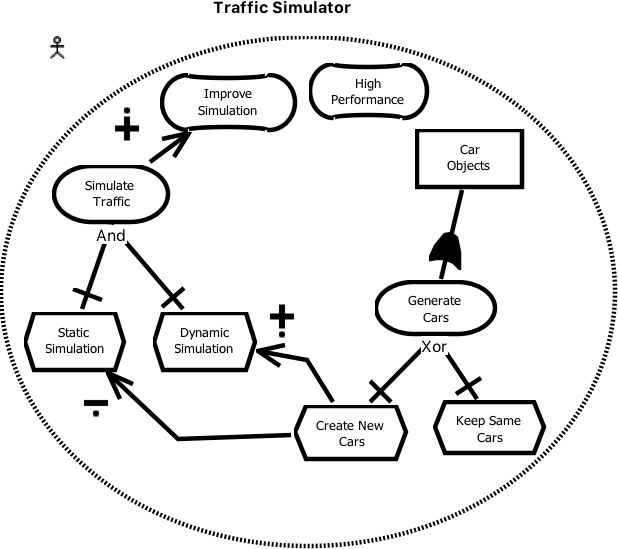
\includegraphics[width=0.5\textwidth]{img/Example1}
\caption{Partial GRL Model of the traffic simulator example}
\label{fig:example-small}
\end{figure} %SG: I changed the figure a bit so that we won't need to change Figure 10. Let me know if you still want to change them according to the above.
%MvZ: The figure looks good to me!

\begin{figure*}[ht]
\centering
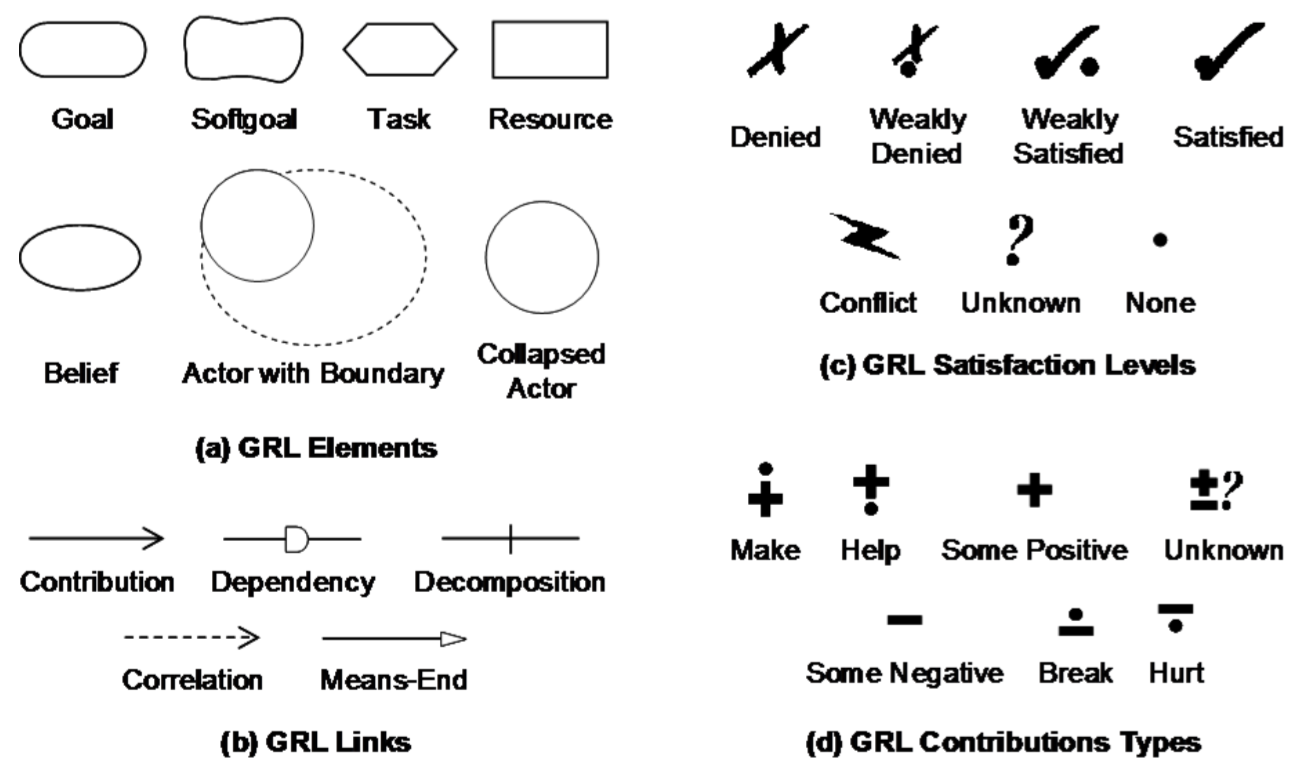
\includegraphics[scale=0.6]{img/grl_legend}
\caption{Basic elements and relationships of GRL}
\label{fig:grl_legend}
\end{figure*}

Figure~\ref{fig:example-small} illustrates a simplified GRL diagram from the traffic simulator design exercise. An actor (
\includegraphics[scale=1]{img/actor}) represents a stakeholder of a system or the system itself (\texttt{Traffic Simulator}, Figure~\ref{fig:example-small}). Actors are holders of intentions; they are the active entities in the system or its environment who want goals to be achieved, tasks to be performed, resources to be available, and softgoals to be satisfied. Softgoals (
\includegraphics[scale=1]{img/softgoal}) differentiate themselves from goals (
\includegraphics[scale=1]{img/goal}) in that there is no clear, objective measure of satisfaction for a softgoal whereas a goal is quantifiable, often in a binary way. Softgoals (e.g. \texttt{Improve Simulation}) are often related to non-functional requirements, whereas goals (such as  \texttt{Simulate Traffic}) are related to functional requirements. Tasks (
\includegraphics[scale=1]{img/task}) represent solutions to (or operationalizations of) goals and softgoals. In Figure~\ref{fig:example-small}, we have the two tasks \texttt{Static Simulation} and \texttt{Dynamic Simulation}: if the system can perform both a static and a dynamic simulation, it can achieve goal \texttt{Simulate Traffic}.\todo{F}{S}{Later in the paper this goal is called  \texttt{Simulate} , not \texttt{Simulate Traffic}. \texttt{Simulate Traffic} seems more clear to me.} In order to be achieved or completed, softgoals, goals, and tasks may require resources (
\includegraphics[scale=1]{img/resource}) to be available (e.g., \texttt{Car Objects}). \todo{F}{S,M}{Belief elements are not explained and not in the example. I think it would be good to include them (or at least discuss them), as beliefs allow one to give some sort of rationale for e.g. goals (in fact, one of the reviewers of one of our previous papers argued that beliefs can also be used to capture reasons).}

Different links connect the elements in a GRL model. AND, IOR (Inclusive OR), and XOR (eXclusive OR) decomposition links (
\includegraphics[scale=1]{img/decomposition}) allow an element to be decomposed into sub-elements. In Figure~\ref{fig:example-small}, the goal \texttt{Generate cars} is XOR-decomposed to the tasks \texttt{Create new cars} and \texttt{Keep same cars}, as they are alternative ways of achieving the goal \texttt{Generate Cars}. Contribution links (
\includegraphics[scale=1]{img/contribution}) indicate desired impacts of one element on another element. A contribution link has a qualitative contribution type or a quantitative contribution. Task  \texttt{Create new cars} has a \emph{help} qualitative contribution to the task \texttt{Dynamic Simulation}, and a \emph{hurt} qualitative contribution to the task \texttt{Static Simulation}. Dependency links (
\includegraphics[scale=1]{img/dependency}) model relationships between actors or resources. Here, the goal \texttt{Generate Cars} depends on the resource \texttt{Car Objects}. %SG: I added it to the model but we can also remove it altogether. 
%\todo{Marc}{Sepideh}{Shall we add a dependency relation as well? They don't play a big role in our work..}
%MvZ: It is a bit strange because we say dependencies are between actors but our examples does show this. Perhaps better to leave it out?

GRL is based on $i*$~\cite{Yu:1997:TMR:827255.827807} and the NFR Framework~\cite{chung2012non}, but it is not as restrictive as $i*$. Intentional elements and links can be more freely combined, the notion of agents is replaced with the more general notion of actors, i.e., stakeholders, and a task does not necessarily have to be an activity performed by an actor, but may also describe properties of a solution. GRL has a well-defined syntax and semantics. Furthermore, GRL provides support for providing a scalable and consistent representation of multiple views/diagrams of the same goal model (see~\cite[Ch.2]{Ghanavati2013} for more details). GRL is also linked to Use Case Maps via URNLinks (
\includegraphics[scale=1]{img/urnlink}) which provide traceability between concepts and instances of the goal model and behavioral design models. Multiple views and traceability links are a good fit with our current research: we aim to add traceability links between intentional elements and their underlying arguments. 

GRL has six evaluation algorithms which are semi-automated and allow the analysis of alternatives and design decisions by calculating the satisfaction value of the intentional elements across multiple diagrams quantitatively, qualitatively or in a hybrid way. The satisfaction values from intentional elements in GRL can also be propagated to the elements of Use Case Maps.  jUCMNav, GRL tool-support, also allows for adding new GRL evaluation algorithms~\cite{jUCMNav}. GRL also has the capability to be extended through metadata, links, and external OCL constraints. This allows GRL to be used in many domains without the need to change the whole modeling language. This feature also helps us apply our argumentation to other domains such as compliance, which we explain in more detail in Section~\ref{sect:goalmodeling:openissues}.

The GRL model in Figure~\ref{fig:example-small} shows the softgoals, goals, tasks and the relationship between the different intentional elements in the model. However, the rationales and arguments behind certain intentional elements are not shown in the GRL model. Some of the questions that might be interesting to know about are the following:

\begin{itemize}
	\item Why does actor \texttt{Traffic Simulator} have softgoal \texttt{High Performance}, which is not linked to any of the goals \texttt{Generate Cars} and \texttt{Simulate Traffic}? %SG: I changed this question but let me know if you want to change them back and then change the graph.
	\item What does \texttt{Keep Same Cars} mean?
	\item Why does task \texttt{Create New Cars} contribute negatively to \texttt{Static Simulation} and positively to \texttt{Dynamic Simulation}?
	\item Why does \texttt{Simulate Traffic} AND-decompose into two tasks?
\end{itemize}

These are the type of the questions that we cannot answer by just looking at GRL models. The model in Figure~\ref{fig:example-small} does not contain information about discussions that led to the resulting model, such as various clarification steps for the naming, or alternatives that have been considered for the relationships. With our RationalGRL framework we aim to address this shortcoming.

\subsection{Argument Scheme for Practical Reasoning (PRAS)}
\label{sect:background:pras}

Reasoning about which goals to pursue and actions to take is often referred to as \emph{practical reasoning}, and has been studied extensively in philosophy (e.g. \cite{Raz1978-RAZPR,walton1990}) and artificial intelligence \cite{bratman1987,atkinson2007}. One approach is to capture practical reasoning with argument schemes~\cite{walton1990}. Applying an argument scheme results in an argument in favor of, for example, taking an action. This argument can then be tested with critical questions about, for instance, whether the action is possible given the situation, and a negative answer to such a question leads to a counterargument to the original argument for the action. 

Atkinson and Bench-Capon~\cite{atkinson2007} develop and formalize the \emph{Practical Reasoning Argument Scheme} (PRAS). A slightly adapted version\footnote{The original argument scheme uses different terminology: Atkinson and Bench-Capon say that realizing a goal contributes to some \emph{value}, an interest which an agent may or may not wish to uphold or subscribe to, such as \texttt{High Performance}. In this paper, we use the term \emph{softgoal} to indicate such interests.} of this argument scheme is as follows:

\begin{itemize}
\item[] We have goal $G$,
\item[] Performing action $A$ realizes goal $G$,
\item[] Which will contribute positively to the softgoal $S$
\item[] \textit{Therefore} 
\item[] We should perform action $A$
\end{itemize}

Here, $G$, $A$, and $S$ are variables, which can be instantiated with concrete goals, actions, and softgoals to provide a specific practical argument. For example, a concrete argument about the traffic simulator is as follows: 
\begin{itemize}
\item[] We have goal \texttt{Simulate Traffic},
\item[] Performing action \texttt{Static Simulation} realizes goal \texttt{Simulate Traffic}, 
\item[] Which contributes positively to the softgoal \texttt{Improve Simulation} 
\item[] \textit{Therefore} 
\item[] We should perform action \texttt{Static Simulation}.
\end{itemize}

Practical reasoning is defeasible, in that conclusions which are at one point acceptable can later be rejected because of new information. Atkinson et al.~\cite{atkinson2007} define a set of critical questions that point to typical ways in which a practical argument can be criticized by, for example, questioning the validity of the elements in the scheme or the connections between the elements. Some examples of critical questions are as follows.

%FB: I deleted a few of the critical questions
\begin{enumerate}
\item Will the action realize the desired goal?
\item Are there alternative ways of realizing the same goal or contributing to the same softgoal?
\item Does performing the action have a negative side effect?
\end{enumerate}

These critical questions can point to new arguments that might counter the original argument. Take, for example, critical question 1: if we find that performing a \texttt{Static Simulation} actually does not realize goal \texttt{Simulate Traffic}, we can form a counter-argument. Another way to criticize an argument for an action is to suggest an alternative action that realizes the same goal (question 2). For example, we can argue that performing a \texttt{Dynamic Simulation} also realizes the goal \texttt{Simulate Traffic} on its own. Finally, it is possible that performing an action has a negative side effect (critical question 3). For example, while the action \texttt{Create New Cars} realizes the goal \texttt{Generate Cars}, it has a negative side effect, namely hurting \texttt{Static Simulation}: having the simulation constantly create new cars is a functionality that does not allow for a static simulation. 

%FB: I extended the example and put the figure back in. Note that this is just to explain argumentation, not to reason about the model in 2.2. Putting explicit text in the example makes it more clear.

In argumentation, counterarguments are said to \emph{attack} the original arguments (and sometimes vice versa). In the work of Atkinson et al.~\cite{atkinson2007}, arguments and their attacks are captured as an \emph{argumentation framework} of arguments and attack relations. Given an argumentation framework, we can compute which arguments are accepted and which are rejected using different argumentation semantics~\cite{Dung1995}\footnote{Formal definitions of argumentation frameworks and semantics will be given in section \ref{sect:gmas}. In this section, we will briefly discuss the intuitions behind these concepts.}. Figure \ref{fig:pras:example} shows an argumentation framework with three arguments from the traffic simulation example, where arguments are rendered as boxes and attack relations as arrows. There are two slightly simplified practical reasoning arguments based on PRAS: argument A1 for \texttt{Keep Same Cars} and argument A2 for \texttt{Create New Cars}. Argument A2 proposes an alternative way of realizing the same goal \texttt{Generate Cars} with respect to argument A1 and vice versa (cf. critical question 2), so A1 and A2 mutually attack each other, denoted by the double-headed arrow between A1 and A2. Argument A3 says that \texttt{Create New Cars} has a negative effect on \texttt{Static Simulation}, so A3 attacks A2, as it points to a negative side-effect of \texttt{Create new cars} (critical question 3). 

\begin{figure}[ht!]
\centering
\begin{tikzpicture}
        \node[minimum size=1cm] (att3) [argNodeIN] at (-0.5,-3.4) {\argtext{A1}{Action \texttt{Keep Same Cars} realizes goal \texttt{Generate Cars}\\ \emph{\underline{Therefore}} we should perform \texttt{Keep Same Cars}}};
        \node[minimum size=1cm] (att1) [argNodeOUT] at (-0.5,0) {\argtext{A2}{Action \texttt{Create New Cars} realizes goal \texttt{Generate Cars}\\ \emph{\underline{Therefore}} we should perform \texttt{Create New Cars}}};
        \node[minimum size=1cm] (att2) [argNodeIN] at (3.5,0) {\argtext{A3}{\texttt{Create New Cars} has a negative effect on \texttt{Static Simulation}}};
         \path
    (att2) edge [attackLink] (att1)
    (att1) edge [attackLink,<->] (att3);
\end{tikzpicture}
\caption{Arguments and attacks in the traffic simulation example.}
\label{fig:pras:example}
\end{figure}

Given an argumentation framework, the acceptability of arguments can be determined according to the appropriate argumentation semantics~\cite{Dung1995}. The intuition is that an argument is acceptable if it is \emph{undefeated}, that is, any argument that attacks it, is itself defeated. In the argumentation framework in Figure~\ref{fig:pras:example}, argument A3 is undefeated because it has no attackers. This makes A2 defeated (indicated by the lighter grey color of A2), because its attacker A3 is undefeated. A1 is then also undefeated, since its only attacker, A2, is defeated by A3. Thus, the set of undefeated (acceptable) arguments given the argumentation framework in Figure~\ref{fig:pras:example} is $\{$A1, A3$\}$.


\subsection{Combining PRAS and GRL}
\label{sect:background:pras:motivation}

%FB: I discuss our previous work on RationalGRL here now (used to be in intro), and I discuss why the approach we take in this paper is different from the approach in our previous work.  

In previous work on the RationalGRL framework~\cite{vanzee-etal:renext2015,vanZee-etal:er2016}, we have explored one way of combining PRAS and GRL. In this work, which takes a similar approach to \cite{Jureta:RE2008}, argument diagrams are translated to GRL models (an automatic translation tool is discussed in~\cite{vanZee-etal:comma2016}). The argument diagrams are complex practical reasoning arguments, where the premises are the goals and the conclusion is some action we need to perform to realize those goals. Thus, we have essentially two complex diagrams, a practical reasoning argument diagram and a GRL goal diagram, and a mapping between them. 

Connecting argumentation and goal modelling by providing a mapping between two types of diagram was, in our opinion, ultimately an unsatisfying solution given the problems and requirements described in Section \ref{sect:introduction}. One problem is that the argument diagram is at least as complex as the GRL diagram, so any stakeholder trying to understand the discussion thus far has to parse two complex diagrams containing goals, alternative solutions, tasks, and so forth. Furthermore, in our previous work we did not provide the specific critical questions for goal models (see Section \ref{sect:gmas}). This meant that any counterargument had to be constructed from scratch, as no guidance was given as to possible ways to criticize a GRL model. So the previous iterations of the RationalGRL framework violated requirement 1: argument diagrams do not closely mirror the actual discussions of stakeholders in which ideas are proposed and challenged. Furthermore, not having specific argument schemes and critical questions for goal modelling makes it hard to develop a guiding methodology for the use of argumentation in goal modelling (requirement 4). 

In the current version of GRL, we do not literally take the Practical Reasoning Argument Scheme and its critical questions - this would be impossible given that there are elements of the GRL language, such as resources, which cannot be found in PRAS. Furthermore, it is not directly clear whether the critical questions as proposed by Atkinson and Bench-Capon~\cite{atkinson2007} actually apply to GRL models. Therefore, we develop our own set of argument schemes and critical questions in Section~\ref{sect:gmas} by analyzing transcripts of discussions about the traffic simulator. Before doing so, we give an overview of our framework in the next section.
